\documentclass[nofonts,]{tufte-handout}

% ams
\usepackage{amssymb,amsmath}

\usepackage{ifxetex,ifluatex}
\usepackage{fixltx2e} % provides \textsubscript
\ifnum 0\ifxetex 1\fi\ifluatex 1\fi=0 % if pdftex
  \usepackage[T1]{fontenc}
  \usepackage[utf8]{inputenc}
\else % if luatex or xelatex
  \makeatletter
  \@ifpackageloaded{fontspec}{}{\usepackage{fontspec}}
  \makeatother
  \defaultfontfeatures{Ligatures=TeX,Scale=MatchLowercase}
  \makeatletter
  \@ifpackageloaded{soul}{
     \renewcommand\allcapsspacing[1]{{\addfontfeature{LetterSpace=15}#1}}
     \renewcommand\smallcapsspacing[1]{{\addfontfeature{LetterSpace=10}#1}}
   }{}
  \makeatother
\fi

% graphix
\usepackage{graphicx}
\setkeys{Gin}{width=\linewidth,totalheight=\textheight,keepaspectratio}

% booktabs
\usepackage{booktabs}

% url
\usepackage{url}

% hyperref
\usepackage{hyperref}

% units.
\usepackage{units}


\setcounter{secnumdepth}{-1}

% citations
\usepackage{natbib}
\bibliographystyle{plainnat}

%% tint override
\setcitestyle{round} 

% pandoc syntax highlighting

% longtable

% multiplecol
\usepackage{multicol}

% strikeout
\usepackage[normalem]{ulem}

% morefloats
\usepackage{morefloats}


% tightlist macro required by pandoc >= 1.14
\providecommand{\tightlist}{%
  \setlength{\itemsep}{0pt}\setlength{\parskip}{0pt}}

% title / author / date
\title{Causality}
\author{Daniel Kaplan}
\date{2019-04-22}

%% -- tint overrides
%% fonts, using roboto (condensed) as default
\usepackage[sfdefault,condensed]{roboto}
%% also nice: \usepackage[default]{lato}

%% colored links, setting 'borrowed' from RJournal.sty with 'Thanks, Achim!'
\RequirePackage{color}
\definecolor{link}{rgb}{0.1,0.1,0.8} %% blue with some grey
\hypersetup{
  colorlinks,%
  citecolor=link,%
  filecolor=link,%
  linkcolor=link,%
  urlcolor=link
}

%% macros
\makeatletter

%% -- tint does not use italics or allcaps in title
\renewcommand{\maketitle}{%     
  \newpage
  \global\@topnum\z@% prevent floats from being placed at the top of the page
  \begingroup
    \setlength{\parindent}{0pt}%
    \setlength{\parskip}{4pt}%
    \let\@@title\@empty
    \let\@@author\@empty
    \let\@@date\@empty
    \ifthenelse{\boolean{@tufte@sfsidenotes}}{%
      %\gdef\@@title{\sffamily\LARGE\allcaps{\@title}\par}%
      %\gdef\@@author{\sffamily\Large\allcaps{\@author}\par}%
      %\gdef\@@date{\sffamily\Large\allcaps{\@date}\par}%
      \gdef\@@title{\begingroup\fontseries{b}\selectfont\LARGE{\@title}\par}%
      \gdef\@@author{\begingroup\fontseries{l}\selectfont\Large{\@author}\par}%
      \gdef\@@date{\begingroup\fontseries{l}\selectfont\Large{\@date}\par}%
    }{%
      %\gdef\@@title{\LARGE\itshape\@title\par}%
      %\gdef\@@author{\Large\itshape\@author\par}%
      %\gdef\@@date{\Large\itshape\@date\par}%
      \gdef\@@title{\begingroup\fontseries{b}\selectfont\LARGE\@title\par\endgroup}%
      \gdef\@@author{\begingroup\fontseries{l}\selectfont\Large\@author\par\endgroup}%
      \gdef\@@date{\begingroup\fontseries{l}\selectfont\Large\@date\par\endgroup}%
    }%
    \@@title
    \@@author
    \@@date
  \endgroup
  \thispagestyle{plain}% suppress the running head
  \tuftebreak% add some space before the text begins
  \@afterindentfalse\@afterheading% suppress indentation of the next paragraph
}

%% -- tint does not use italics or allcaps in section/subsection/paragraph
\titleformat{\section}%
  [hang]% shape
  %{\normalfont\Large\itshape}% format applied to label+text
  {\fontseries{b}\selectfont\Large}% format applied to label+text
  {\thesection}% label
  {1em}% horizontal separation between label and title body
  {}% before the title body
  []% after the title body

\titleformat{\subsection}%
  [hang]% shape
  %{\normalfont\large\itshape}% format applied to label+text
  {\fontseries{m}\selectfont\large}% format applied to label+text
  {\thesubsection}% label
  {1em}% horizontal separation between label and title body
  {}% before the title body
  []% after the title body

\titleformat{\paragraph}%
  [runin]% shape
  %{\normalfont\itshape}% format applied to label+text
  {\fontseries{l}\selectfont}% format applied to label+text
  {\theparagraph}% label
  {1em}% horizontal separation between label and title body
  {}% before the title body
  []% after the title body

%% -- tint does not use italics here either
% Formatting for main TOC (printed in front matter)
% {section} [left] {above} {before w/label} {before w/o label} {filler + page} [after]
\ifthenelse{\boolean{@tufte@toc}}{%
  \titlecontents{part}% FIXME
    [0em] % distance from left margin
    %{\vspace{1.5\baselineskip}\begin{fullwidth}\LARGE\rmfamily\itshape} % above (global formatting of entry)
    {\vspace{1.5\baselineskip}\begin{fullwidth}\fontseries{m}\selectfont\LARGE} % above (global formatting of entry)
    {\contentslabel{2em}} % before w/label (label = ``II'')
    {} % before w/o label
    {\rmfamily\upshape\qquad\thecontentspage} % filler + page (leaders and page num)
    [\end{fullwidth}] % after
  \titlecontents{chapter}%
    [0em] % distance from left margin
    %{\vspace{1.5\baselineskip}\begin{fullwidth}\LARGE\rmfamily\itshape} % above (global formatting of entry)
    {\vspace{1.5\baselineskip}\begin{fullwidth}\fontseries{m}\selectfont\LARGE} % above (global formatting of entry)
    {\hspace*{0em}\contentslabel{2em}} % before w/label (label = ``2'')
    {\hspace*{0em}} % before w/o label
    %{\rmfamily\upshape\qquad\thecontentspage} % filler + page (leaders and page num)
    {\upshape\qquad\thecontentspage} % filler + page (leaders and page num)
    [\end{fullwidth}] % after
  \titlecontents{section}% FIXME
    [0em] % distance from left margin
    %{\vspace{0\baselineskip}\begin{fullwidth}\Large\rmfamily\itshape} % above (global formatting of entry)
    {\vspace{0\baselineskip}\begin{fullwidth}\fontseries{m}\selectfont\Large} % above (global formatting of entry)
    {\hspace*{2em}\contentslabel{2em}} % before w/label (label = ``2.6'')
    {\hspace*{2em}} % before w/o label
    %{\rmfamily\upshape\qquad\thecontentspage} % filler + page (leaders and page num)
    {\upshape\qquad\thecontentspage} % filler + page (leaders and page num)
    [\end{fullwidth}] % after
  \titlecontents{subsection}% FIXME
    [0em] % distance from left margin
    %{\vspace{0\baselineskip}\begin{fullwidth}\large\rmfamily\itshape} % above (global formatting of entry)
    {\vspace{0\baselineskip}\begin{fullwidth}\fontseries{m}\selectfont\large} % above (global formatting of entry)
    {\hspace*{4em}\contentslabel{4em}} % before w/label (label = ``2.6.1'')
    {\hspace*{4em}} % before w/o label
    %{\rmfamily\upshape\qquad\thecontentspage} % filler + page (leaders and page num)
    {\upshape\qquad\thecontentspage} % filler + page (leaders and page num)
    [\end{fullwidth}] % after
  \titlecontents{paragraph}% FIXME
    [0em] % distance from left margin
    %{\vspace{0\baselineskip}\begin{fullwidth}\normalsize\rmfamily\itshape} % above (global formatting of entry)
    {\vspace{0\baselineskip}\begin{fullwidth}\fontseries{m}\selectfont\normalsize\rmfamily} % above (global formatting of entry)
    {\hspace*{6em}\contentslabel{2em}} % before w/label (label = ``2.6.0.0.1'')
    {\hspace*{6em}} % before w/o label
    %{\rmfamily\upshape\qquad\thecontentspage} % filler + page (leaders and page num)
    {\upshape\qquad\thecontentspage} % filler + page (leaders and page num)
    [\end{fullwidth}] % after
}{}

  
\makeatother



\begin{document}

\maketitle




\hypertarget{activities}{%
\subsection{Activities}\label{activities}}

\begin{itemize}
\tightlist
\item
  \href{/lessons/intervention-and-prediction/}{Intervention and
  prediction}
\item
  \href{/lessons/experiment-and-causality/}{Experiment and causality}
\end{itemize}

\hypertarget{learning-objectives}{%
\subsection{Learning objectives}\label{learning-objectives}}

\hypertarget{additional-sections}{%
\subsection{Additional sections}\label{additional-sections}}

\begin{itemize}
\item
\item
  \protect\hyperlink{orientation}{Instructor orientation}
\item
  \protect\hyperlink{role}{Role in statistical practice}
\item
  \protect\hyperlink{discussion}{Classroom discussion}
\item
  \protect\hyperlink{active}{Tips for an active classroom}
\item
  \protect\hyperlink{prereqs}{Student pre-requisites}
\item
  \protect\hyperlink{pitfalls}{Pitfalls}
\end{itemize}

\hypertarget{orientation-for-instructors}{%
\section{Orientation for
instructors}\label{orientation-for-instructors}}

There is an epigram that is familiar to \emph{all} statistics
instructors:

\begin{quote}
\emph{Correlation is not causation.}
\end{quote}

Put on a more explicit logical footing, this is equivalent to:

\begin{quote}
\emph{Correlation does not imply causation.}
\end{quote}

But as familiar as this epigram is, it's wrong. We legitimately can say
this:

\begin{quote}
\emph{No causation implies no correlation.}
\end{quote}

The ``no correlation'' part of this is pretty easy. We have many
statistical techniques for working with two variables X and Y --
t-tests, regression, etc -- that can establish correlation. So by ``no
correlation'' we mean that any of these tests have failed to demonstrate
a correlation.

But ``no causation'' is more subtle. Knowing what this means requires a
bit of formalism. The formalism we will use is that of diagrams:
directed acyclic graphs.

Here are several:

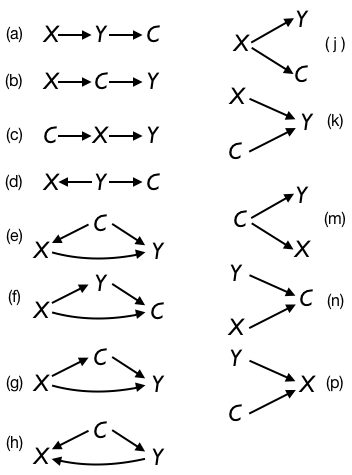
\includegraphics{../../static../../static../../static/images/many-dags.png}

We can define ``no causation'' in terms of these graphs. Here's a useful
approximation: The procedure is to imagine putting ants into one of the
nodes of the graph. And these imaginary ants can (and will!) move only
along the arrows in the direction of the arrowhead. The ants can't walk
against the flow of the arrow.

By ``no causation'' between X and Y we mean that there is no node from
which ants can get to both X and Y.

This definition works well enough so long as the variables X, Y, and C
are left to their own devices, being caused according to the arrows in
the diagram. But if we intervene, say holding some node at a constant
value, then we might close down an otherwise legitimate along-the-arrows
pathway involving X and Y, or we might even open up a pathway, like that
through C in diagram (n), that ordinary wouldn't let ants get to X and Y
from C. Such a situation is called a ``collider.''

It's starting to get complicated. I think this is part of the motivation
for the traditional canon of introductory statistics, namely:

\begin{enumerate}
\def\labelenumi{\arabic{enumi}.}
\tightlist
\item
  Correlation is not causation.
\item
  Experimental intervention is the only way to establish causation.
\item
  In an experiment we impose variability on X and look for correlated
  variability in Y.
\end{enumerate}

This is a nice story, but it's incomplete. For example, not all
experiments involve imposing variability on X. An experimental
intervention could be holding some other variable \emph{constant}. And
there are three ways to hold a variable constant:

\begin{enumerate}
\def\labelenumi{\alph{enumi}.}
\tightlist
\item
  Physically pin the variable to a constant value, e.g.~by regulating
  the temperature in an experimental chamber.
\item
  Select a subset of cases from the data for which the variable happens
  to be at a constant value.
\item
  In a model, include the variable to be held constant among the
  explanatory variables. Consequently, when using the model to generate
  simulated data, we can intervene to hold that variable constant.
  Effectively, we build a model of the world and do experiments on that
  model.
\end{enumerate}

\begin{enumerate}
\def\labelenumi{(\alph{enumi})}
\tightlist
\item
  and (b) are the most compelling, because we can't really know if the
  model in (c) actually represents the real-world system.
\end{enumerate}

What we miss out entirely in the canonical intro stats curriculum is the
kind of experiment that involves holding variables constant. Such
experiments can actually be used to reject hypotheses about causal
networks. If we observe a correlation when the hypothetical network
(augmented, perhaps, by holding variables constant) says we shouldn't,
we can reject the hypothesis. Or if we see no correlation when the
network says we should see one, we can reject the hypothesis. This
process of elimination, involving experiments where variables are held
constant, can sometimes resolve a dispute between two rival hypotheses.

Going back to the statement that ``no causation implies no
correlation,'' we can take the contrapositive to arrive at this, more
meaningful statement:

\begin{quote}
\emph{Correlation implies causation.}
\end{quote}

It's just that the correlation doesn't by itself distringuish between
rival hypotheses, telling us, for example, whether X causes Y or the
other way around, or whether there is a common cause shaping both X and
Y. But by doing hold-a-variable-constant experiments, we can distinguish
between different possible arrangements of X, Y, and C.

\hypertarget{role-in-statistical-practice}{%
\subsection{Role in statistical
practice}\label{role-in-statistical-practice}}

Causation is an important issue in describing how systems work or
deciding on what kind of intervention will be effective.

There are many situations where an impose-variation experiment is
impossible for practical or ethical reasons. (We'll force this group to
smoke and that group to abstain. An idea not likely to get far.) And so,
it's important to be able to make reasoned judgements about causality.

Consider what happens in practice when we adhere to the ``correlation is
not causation'' motto. At the end of some newspaper article about recent
research showing the health benefits of an herbal preparation there will
be a disclaimer: ``This was an observational study, so no conclusion
about causation can be drawn.'' Good. So why did the newspaper decide
it's worthwhile to publish the story? And what is a reader supposed to
do with the information. The reader is hardly in a position to decide on
causality when the scientific experts doing the study couldn't do so.

Instead, the newspaper should list the variables that were ``held
constant,'' or ``adjusted for,'' or ``controlled for.'' And they should
point out whether there are likely variables that play an important role
in the system that have not been adjusted for.

\hypertarget{learning-objectives-1}{%
\subsection{Learning objectives}\label{learning-objectives-1}}

\begin{enumerate}
\def\labelenumi{\arabic{enumi}.}
\tightlist
\item
  Understand that an observed correlation, on its own, doesn't
  distinguish among specific causal arrangements.
\item
  Understand that doing an intervention experiment (one where
  variability is imposed on X that is independent of all other sources
  of variability) can reveal a causal connection from X to Y, if a
  correlation is observed between X and Y in the experimental data.
\item
  Be able to make sense of the common practice in studies of ``holding
  constant'' or ``adjusting for.''
\end{enumerate}

\hypertarget{student-tasks-and-activities}{%
\subsection{Student tasks and
activities}\label{student-tasks-and-activities}}

See the activities listed at the top of this document.

\hypertarget{assessment-items}{%
\subsection{Assessment items}\label{assessment-items}}

See the activities listed at the top of this document.

\hypertarget{pushing-the-envelopeadvancing-the-field}{%
\subsection{Pushing the envelope/advancing the
field}\label{pushing-the-envelopeadvancing-the-field}}

Just by talking about causation in a way that reflects informed
professional practice in many fields, students will be able to see that
what they learn in statistics is not in conflict with that practice.

\begin{center}\rule{0.5\linewidth}{\linethickness}\end{center}

Danny Kaplan, version 0.3, Tue May 28 14:12:18 2019



\end{document}
